
\documentclass[template=tabling,81pt,headonall]{azmoon}
\usepackage{xepersian}
\usepackage{amsfonts}
\usepackage{graphicx}
\usepackage{svg}
\svgpath{ {./images/} }
\graphicspath{ {./images/} }
\settextfont{Yas}
\setdigitfont{A Iranian Sans}
\usepackage{fontawesome5}

\printanswers
    \teacher{محمد صالح علی اکبری}
    \teachertitle{دبیر}
    \city{گناباد}
    \schooltitle{دبیرستان}
    \school{شهید جوانبخت}
    \grade{هشتم (نمونه ب)}
    \branch{نمونه ب}
    \topic{ریاضی}
    \examdate{۲۳ مهر ۱۴۰۵}
    \answertime{۵۰ دقیقه}
    \begin{document}
	\begin{questions}
		\nointerlineskip%
		\vskip-\baselineskip
		\question[6]{%
\textbf{حاصل هر یک از عبارت‌های زیر را به دست آورید:}
\begin{LTR}
\begin{tabular*}{\linewidth}{@{\extracolsep{\fill}}lll}
الف) $42 + 53 = $ & ب) $75 - 38 = $ & ج) $350 - 120 = $ \\\\[0.5em]
د) $(+18) + (-24) = $ & هـ) $(-14) - (+6) = $ & و) $(-7) - (-11) + (-5) = $
\end{tabular*}
\end{LTR}}\question[4]{%
\textbf{به پرسش‌های زیر دربارهٔ عددهای گویا پاسخ دهید:}\\[0.2em]
الف) عددهای $+1\dfrac{1}{3}$ و $-\dfrac{5}{2}$ را روی محور زیر با رسم شکل یا علامت مشخص کنید:\\[0.15em]
\centerline{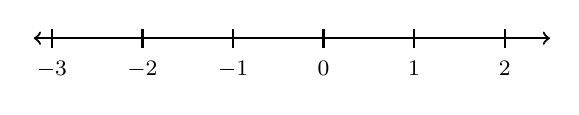
\begin{tikzpicture}[x=1.15cm]
\draw[<->,thick] (-3.2,0) -- (2.5,0);
\foreach \x in {-3,-2,-1,0,1,2} \draw[thick] (\x,0.12) -- (\x,-0.12) node[below=1pt] {\footnotesize $\x$};
\end{tikzpicture}}\\[0.2em]
ب) معکوس عدد صفر چیست؟ چرا؟ \dotfill \quad معکوس $-1\dfrac{1}{4}$: \dotfill \\\\[0.3em]
ج) بین دو عدد گویا $-\dfrac{1}{5}$ و $+\dfrac{2}{5}$ دو عدد گویای دلخواه بنویسید: \dotfill \\\\[0.3em]
د) در جای خالی علامت مناسب ($>$ یا $<$ یا $=$) قرار دهید: \hfill 
$-0.6 \quad \bigcirc \quad -\dfrac{3}{5}$}\question[5]{%
\textbf{حاصل جمع و تفریق‌های زیر را به دست آورده و در صورت امکان ساده کنید:}
\begin{LTR}
\begin{tabular*}{\linewidth}{@{\extracolsep{\fill}}lll}
الف) $\left(+\dfrac{5}{8}\right) + \left(-\dfrac{7}{8}\right) = $ & 
ب) $\left(-\dfrac{3}{5}\right) - \left(-\dfrac{1}{2}\right) = $ & 
ج) $-3 + 1\dfrac{2}{5} = $
\end{tabular*}
\end{LTR}‌
\\‌
\\}\question[5]{%
\textbf{حاصل عبارت‌های زیر را به دست آورید:}
\begin{LTR}
\begin{tabular*}{\linewidth}{@{\extracolsep{\fill}}ll}
الف) $\left(-\dfrac{15}{8}\right) \times \left(-\dfrac{4}{5}\right) = $ & 
ب) $\left(+\dfrac{7}{12}\right) \div \left(-\dfrac{14}{3}\right) = $ \\\\[1.8em]
\multicolumn{2}{l}{ج) $-\dfrac{2}{3} \times \left(\dfrac{3}{4} - \dfrac{1}{2}\right) = $}
\end{tabular*}
\end{LTR}‌
\\}\end{questions}
    \end{document}
    